\chapter{Opis działania aplikacji}

Rozdział opisuje logikę funkcjonowania aplikacji poprzez opisanie jej poszczególnych funkcjonalności oraz przedstawienie kodu.

\section{Struktura i logika aplikacji}
Oprogramowanie zostało zaprojektowane w sposób modułowy, co ułatwia zarządzanie kodem i wprowadzanie ewentualnych poprawek w przyszłości. Główna aktywność zarządza procesem pobierania danych, podczas gdy dedykowana klasa ustawień odpowiada za interakcję z pamięcią trwałą urządzenia. Dzięki takiemu podziałowi, zmiana adresu IP lub interwału czasowego w ustawieniach jest natychmiastowo wykrywana przez moduł komunikacyjny, co pozwala na płynne dostosowanie pracy aplikacji bez konieczności jej restartowania.

\subsection{Struktura klas}

Diagram klas na Rysunku \ref{fig:klasy} pokazuje powiązania między głównymi elementami aplikacji: aktywnościami, modelem danych oraz warstwą komunikacji sieciowej. Pozwala to zrozumieć, jak zbudowana jest struktura programu.
\begin{figure}[H]
    \centering
    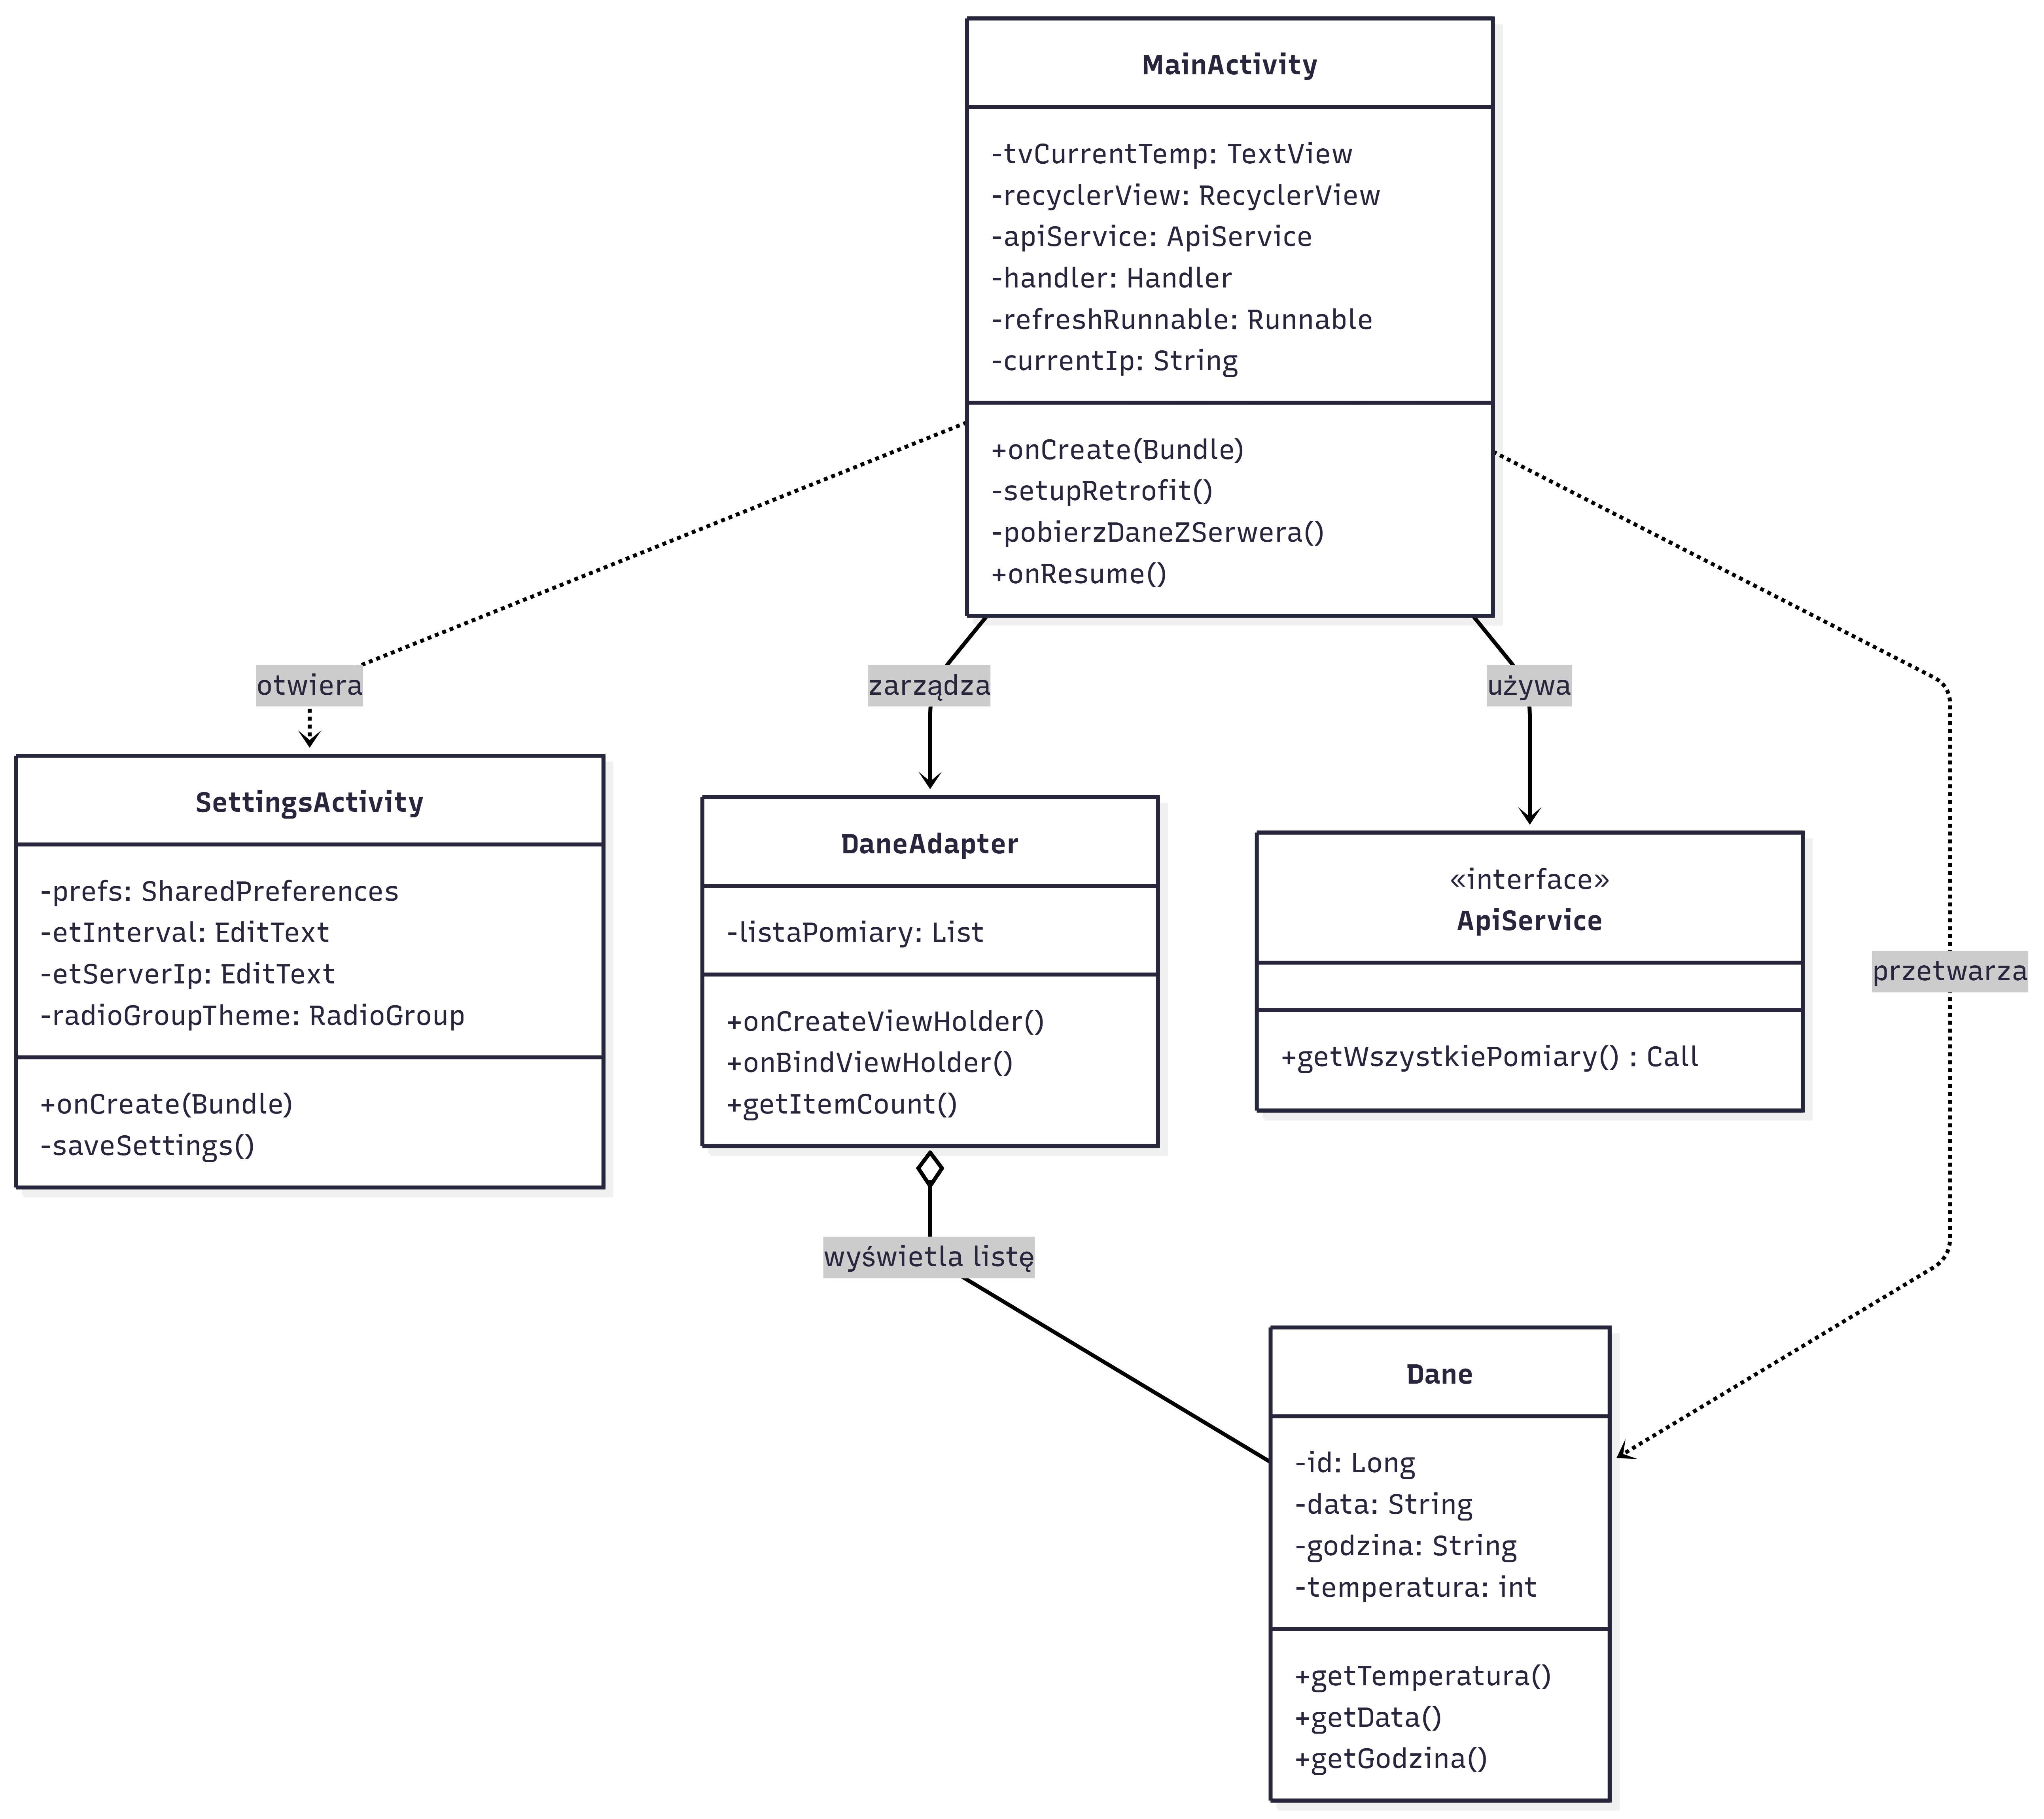
\includegraphics[width=0.7\textwidth]{rysunki/klasy.png} 
    \caption{Diagram Klas (Struktura aplikacji)}
    \label{fig:klasy} % Klucz dla grafiki PNG
    \sourcefig{opracowanie własne}
\end{figure}

\subsection{Przpływ danych}

Diagram sekwencji na Rysunku \ref{fig:dane} przedstawia krok po kroku przebieg komunikacji aplikacji z serwerem i odświeżanie danych. Dzięki temu łatwo prześledzić działanie pętli pobierania informacji.
\begin{figure}[H]
    \centering
    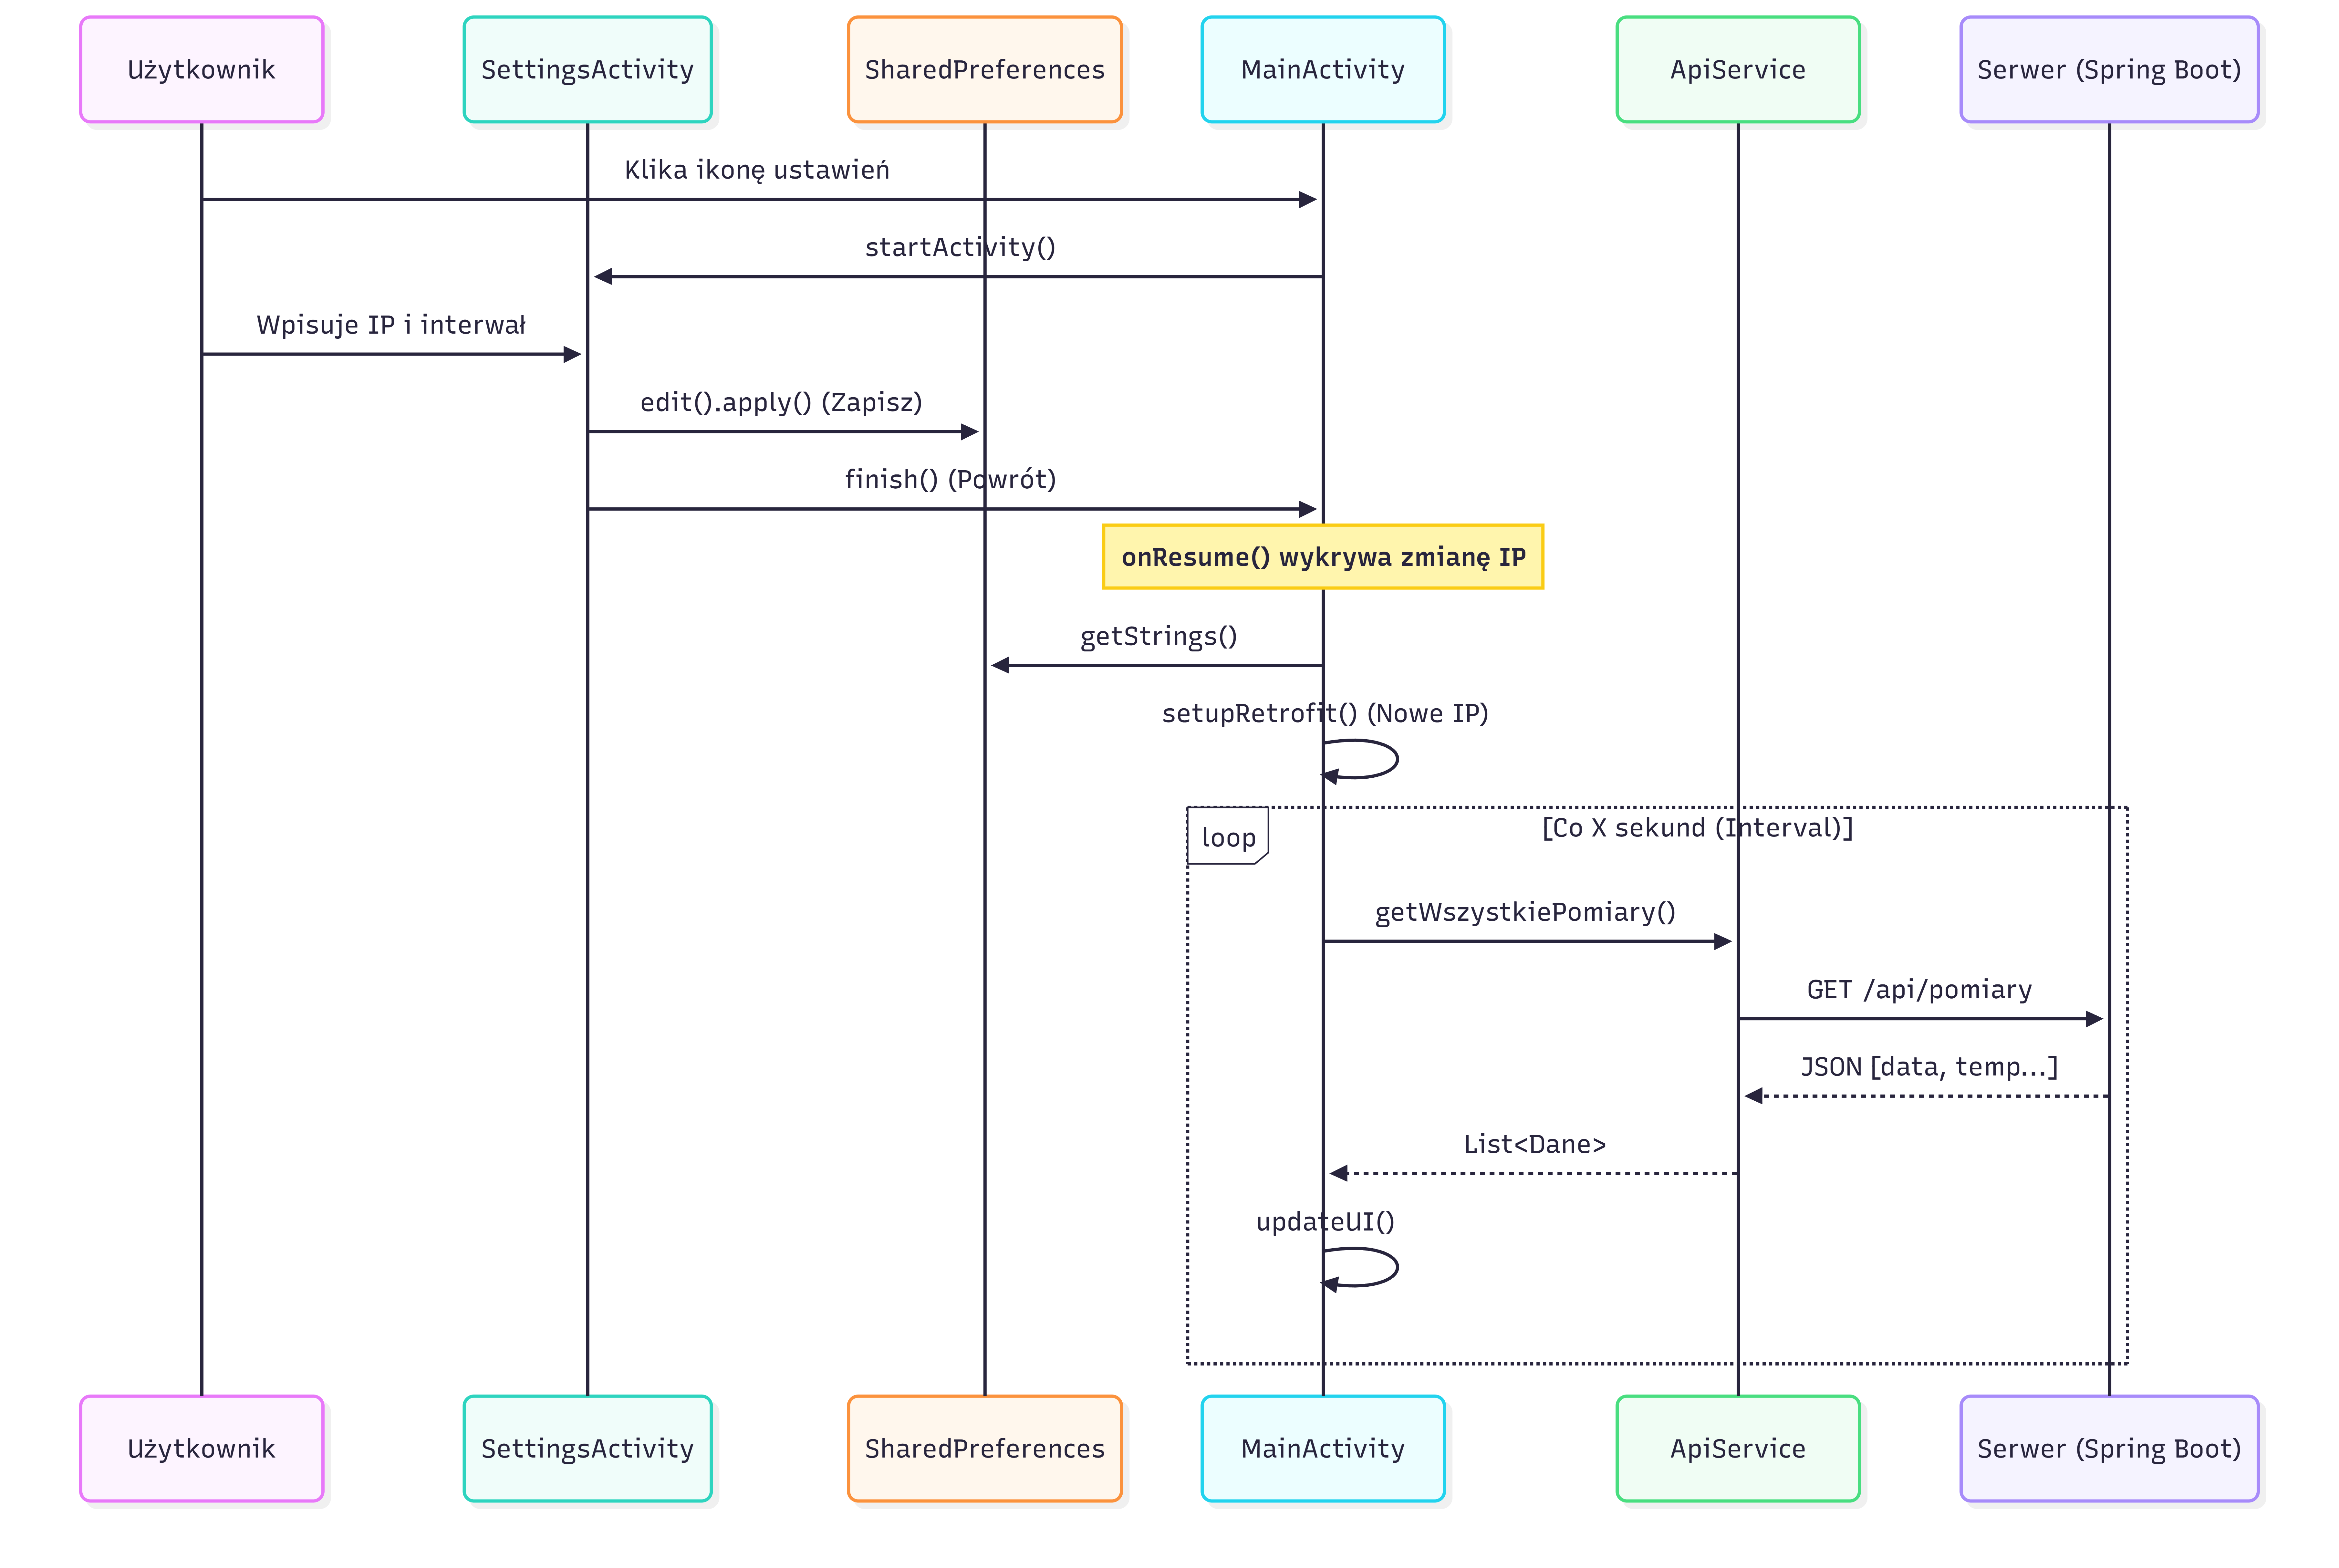
\includegraphics[width=0.7\textwidth]{rysunki/dane.png} 
    \caption{Diagram Sekwencji (Przepływ danych)}
    \label{fig:dane} % Klucz dla grafiki PNG
    \sourcefig{opracowanie własne}
\end{figure}

\section{Interfejs użytkownika}

Warstwa wizualna została podzielona na dwa główne ekrany, które pozwalają na wygodne korzystanie z dostępnych funkcji. Ekran główny skupia się na prezentacji danych, oferując przejrzysty podgląd aktualnych i historycznych odczytów. Ekran ustawień z kolei udostępnia formularze i przełączniki, dzięki którym użytkownik może dostosować aplikację do własnych potrzeb technicznych i estetycznych, dbając o czytelność elementów niezależnie od wybranego motywu graficznego.

\pagebreak

\subsection{Ekran główny}
Ekran główny został zaprojektowany z myślą o intuicyjności i szybkości dostępu do informacji. Centralnym elementem jest duży, wyraźny wskaźnik aktualnej temperatury, który natychmiast przyciąga uwagę użytkownika. Poniżej znajduje się chronologiczna lista wszystkich odczytów, która umożliwia łatwe porównanie bieżących danych z wcześniejszymi pomiarami. Dzięki zastosowaniu komponentu RecyclerView, lista ta jest nie tylko estetyczna, ale także wydajna, nawet przy dużej liczbie wpisów. Rysunek \ref{fig:ekran_glowny} przedstawia interfejs aplikacji, który został zaprojektowany zgodnie z wytycznymi Material Design, zapewniając spójność i nowoczesny wygląd.
\begin{figure}[H]
    \centering
    
\includegraphics[width=0.4\textwidth]{rysunki/1.png} 
    \caption{Ekran główny aplikacji}
    \label{fig:ekran_glowny} % Klucz dla grafiki PNG
    \sourcefig{opracowanie własne przy użyciu emulatora Android Studio}
\end{figure}

\pagebreak

Jak pokazano na rysunku \ref{fig:motyw_ciemny}, poniżej zaprezentowano ekran główny w ciemnym motywie, który jest dostępny w ustawieniach. Dzięki temu użytkownik może dostosować wygląd aplikacji do swoich preferencji, co zwiększa komfort korzystania z niej w różnych warunkach oświetleniowych.
\begin{figure}[H]
    \centering
    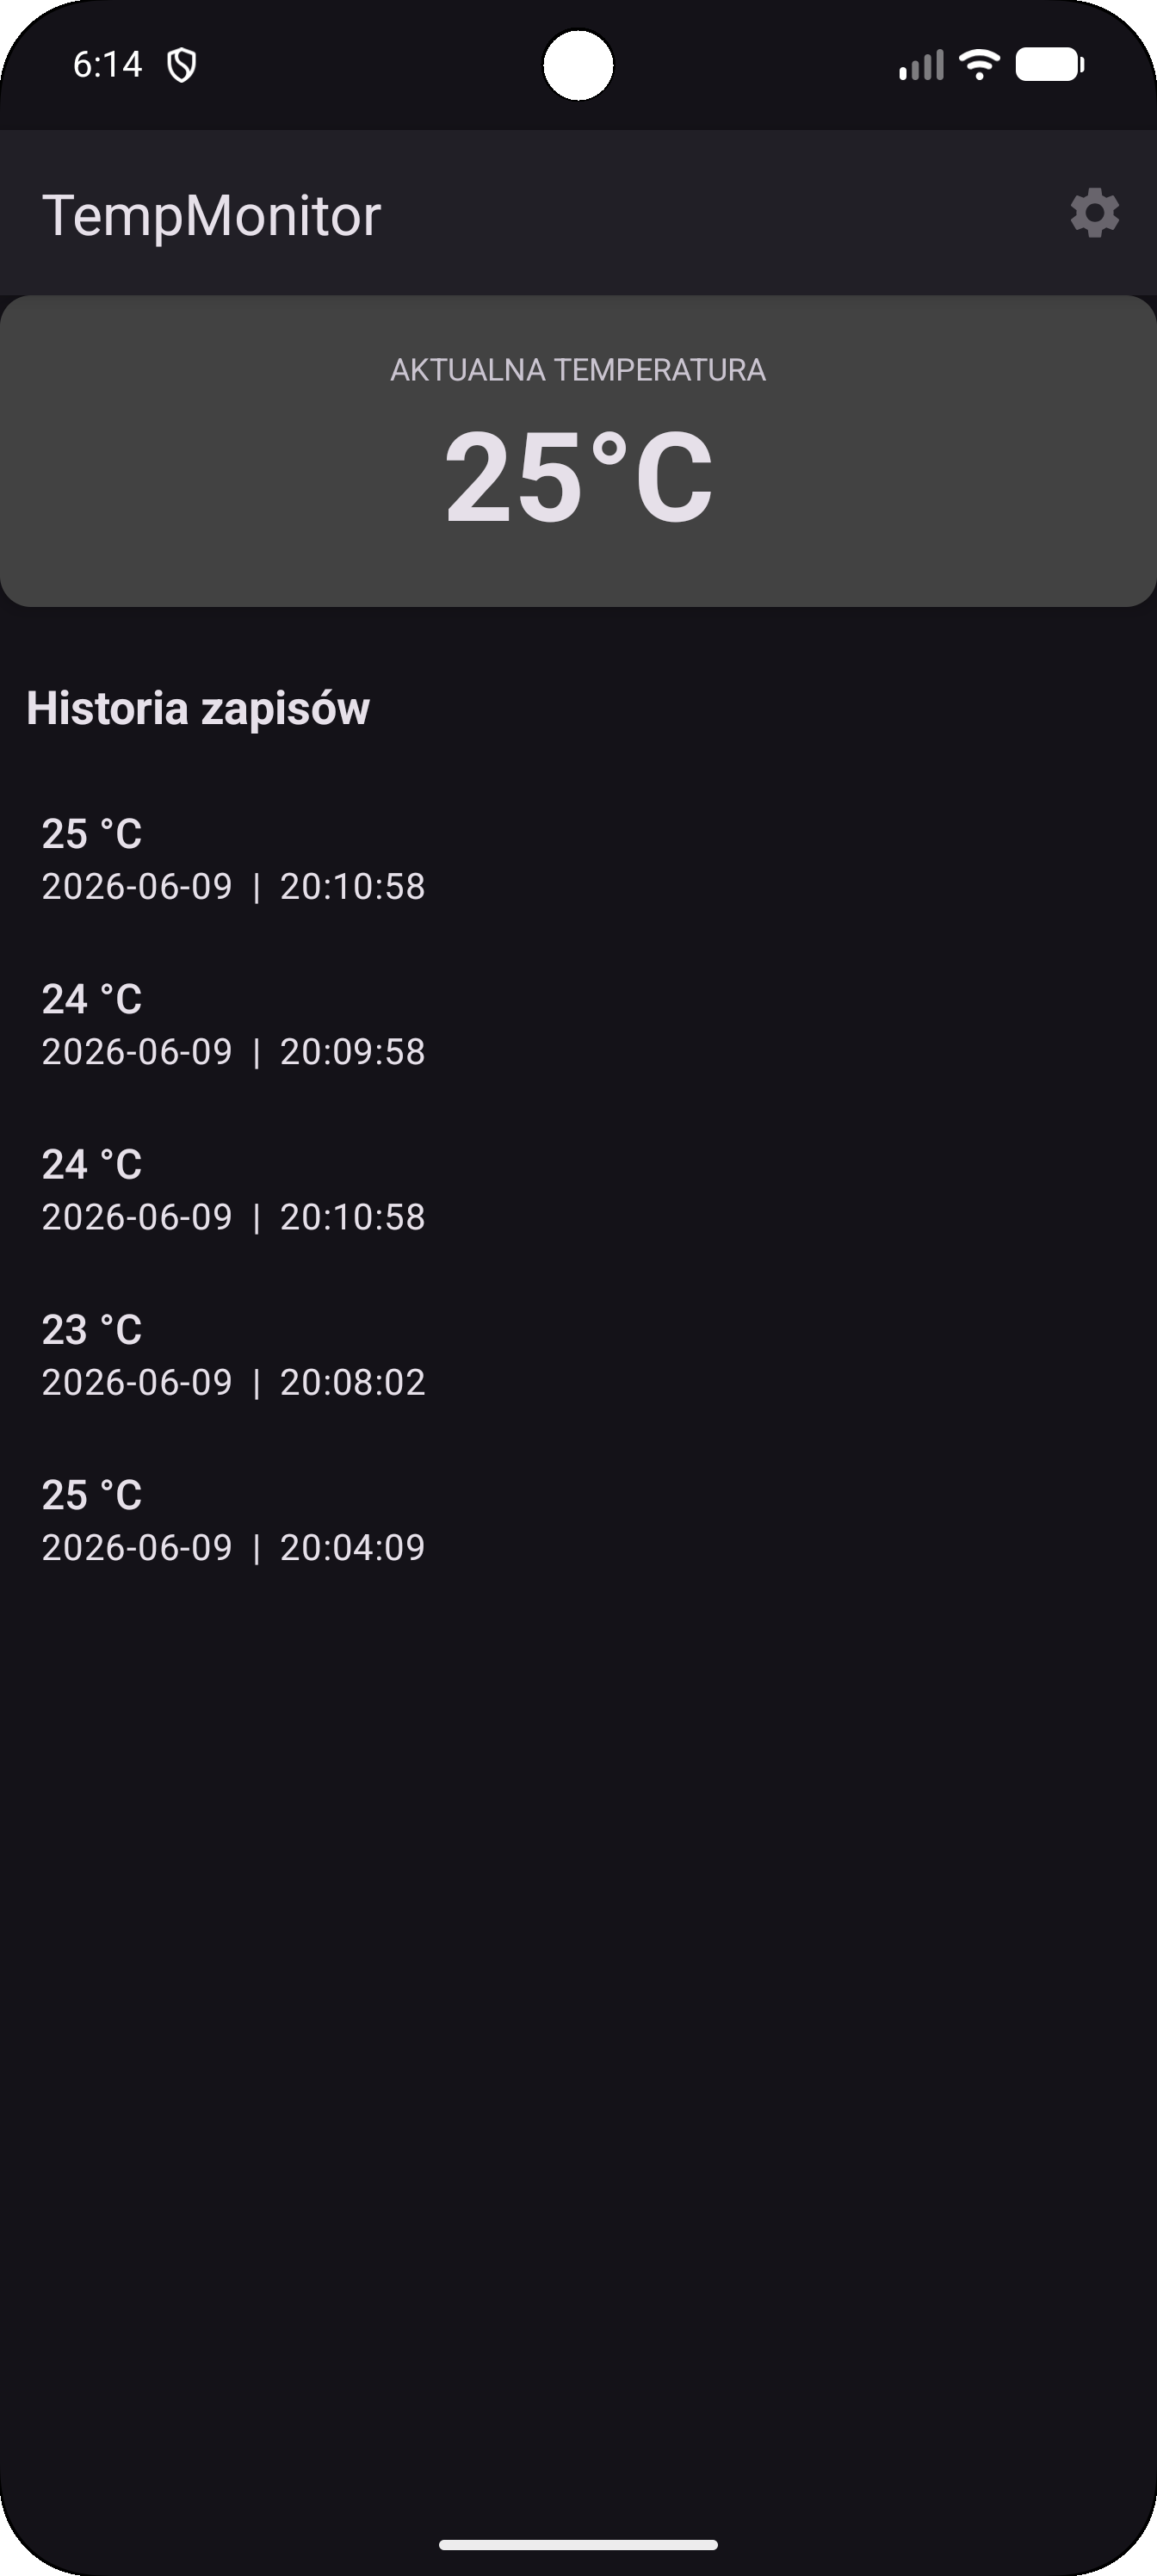
\includegraphics[width=0.4\textwidth]{rysunki/2.png} 
    \caption{Ekran główny aplikacji w ciemnym motywie}
    \label{fig:motyw_ciemny} % Klucz dla grafiki PNG
    \sourcefig{opracowanie własne przy użyciu emulatora Android Studio}
\end{figure}

\pagebreak

\subsection{Ekran ustawień}
Ekran ustawień został zaprojektowany z myślą o maksymalnej funkcjonalności i prostocie obsługi. Użytkownik ma możliwość konfiguracji kluczowych parametrów sieciowych, takich jak adres IP i port serwera, co pozwala na łatwe dostosowanie aplikacji do różnych środowisk sieciowych. Dodatkowo, opcja wyboru motywu graficznego umożliwia personalizację wyglądu interfejsu, co jest szczególnie ważne dla użytkowników preferujących ciemny motyw w warunkach słabego oświetlenia. Rysunek \ref{fig:ekran_ustawien} przedstawia ekran ustawień, który został zaprojektowany zgodnie z wytycznymi Material Design, zapewniając spójność i nowoczesny wygląd.
\begin{figure}[H]
    \centering
    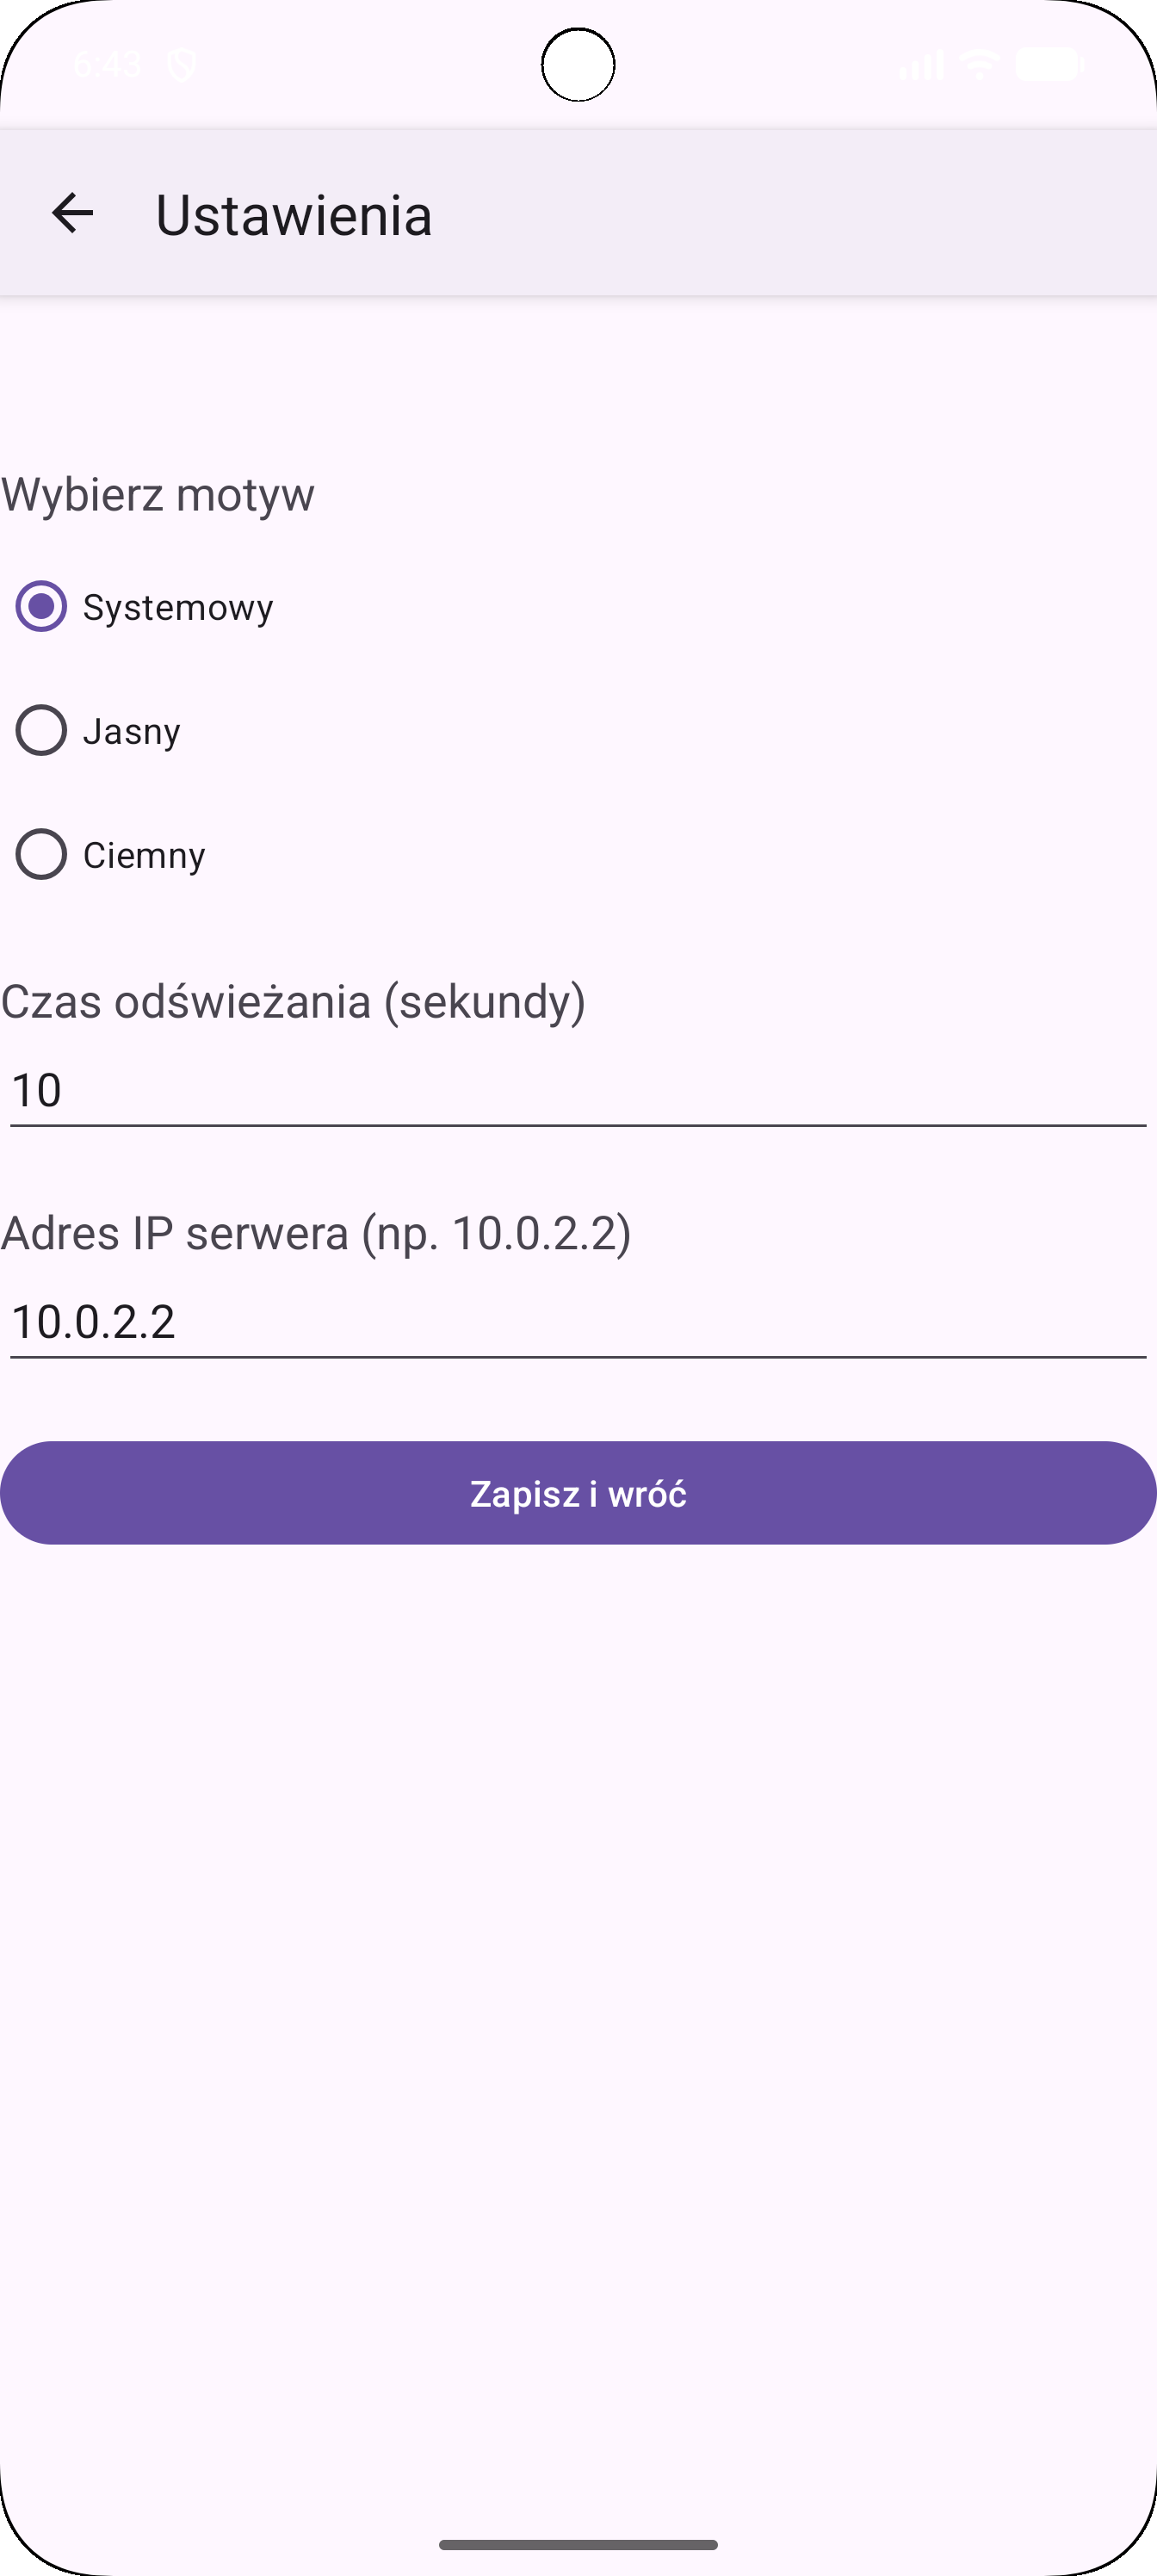
\includegraphics[width=0.4\textwidth]{rysunki/3.png} 
    \caption{Ekran ustawień aplikacji}
    \label{fig:ekran_ustawien} % Klucz dla grafiki PNG
    \sourcefig{opracowanie własne przy użyciu emulatora Android Studio}
\end{figure}

\pagebreak

\section{Pobieranie danych z REST API}
Aplikacja korzysta z biblioteki Retrofit do asynchronicznego pobierania danych. Oznacza to, że pobieranie odbywa się w tle i nie zawiesza ekranu użytkownika.
\begin{lstlisting}[language=Java, caption={Pobieranie danych z API (Fragment ApiService.java)}]
@GET("api/pomiary")
Call<List<Dane>> getWszystkiePomiary();
\end{lstlisting}

\section{Automatyczne odświeżanie co 10 sekund}
Zastosowano mechanizm Handler i Runnable, który tworzy pętlę czasową. Funkcja ta jest inteligentna: uruchamia się, gdy aplikacja jest widoczna, i zatrzymuje, gdy użytkownik ją zminimalizuje.
\begin{lstlisting}[language=Java, caption={Odświeżanie (Fragment MainActivity.java)}]
    refreshRunnable = new Runnable() {
    @Override
    public void run() {
        pobierzDaneZSerwera(); // Wywołanie API
        handler.postDelayed(this, 10000); // Ponowne uruchomienie za 10s
    }
};       
\end{lstlisting}

\section{Logika wyświetlania aktualnej temperatury}
Aplikacja nie potrzebuje osobnego zapytania o jedną temperaturę. Pobiera całą listę, a następnie wybiera z niej ostatni element, aby wyświetlić go jako stan aktualny.
\begin{lstlisting}[language=Java, caption={Wyswietlanie "Aktualnej temperatury" (Fragment MainActivity.java)}]
    if (!daneList.isEmpty()) {
    Dane ostatni = daneList.get(daneList.size() - 1); // Pobranie najnowszego wpisu
    tvCurrentTemp.setText(ostatni.getTemperatura() + "'C");
    Collections.reverse(daneList); // Odwrocenie listy dla historii (najnowsze na gorze)
}
\end{lstlisting}

\section{Wyświetlanie dziennika}
Adapter bierze surowe dane i wstrzykuje je w odpowiednie pola tekstowe w layoucie.
\begin{lstlisting}[language=Java, caption={Wyswietlanie diennika (Fragment DaneAdapter.java)}]
    @Override
    public void onBindViewHolder(@NonNull ViewHolder holder, int position) {
    Dane d = lista.get(position);
    holder.text1.setText(d.getTemperatura() + "'C");
    holder.text2.setText(d.getData() + "  |  " + d.getGodzina());
}
\end{lstlisting}